\chapter{Locality Sensitive Hashing}
\label{chapter:lsh}

\abstract{
In the preceding chapter, we delved into algorithms that inferred the
geometrical shape of a collection of vectors and condensed it into
a navigable structure. In many cases, the algorithms were designed for exact
top-$k$ retrieval, but could be modified to provide guarantees on approximate
search. This section, instead, explores an entirely different idea that is
probabilistic in nature and, as such, is designed specifically for approximate
top-$k$ retrieval from the ground up.
}

\section{Intuition}
\label{section:lsh:intuition}
Let us consider the intuition behind what is known as \emph{Locality Sensitive Hashing}
(LSH)~\citep{lsh} first.
Define $b$ separate ``buckets.'' Now, suppose there exists a mapping $h(\cdot)$
from vectors in $\mathbb{R}^d$ to these buckets, such that every vector is placed into
a single bucket: $h: \mathbb{R}^d \rightarrow [b]$. Crucially, assume that vectors that are closer to each other
according to the distance function $\delta(\cdot, \cdot)$, are more likely to be placed
into the same bucket. In other words, the probability that two vectors collide
increases as $\delta$ decreases.

Considering the setup above, indexing is simply a matter of applying $h$ to
all vectors in the collection $\mathcal{X}$ and making note of the resulting placements.
Retrieval for a query $q$ is also straightforward: Perform exact
search over the data points that are in the bucket $h(q)$.
The reason this procedure works with high probability is because it
is more likely for the mapping $h$ to place $q$ in a bucket that contains
its nearest neighbors, so that an exact search over the $h(q)$ bucket yields the correct
top-$k$ vectors with high likelihood. This is visualized in Figure~\subref*{figure:lsh:intuition:single-dimensional}.

\begin{figure}[t]
    \centering
    \subfloat[]{
        \label{figure:lsh:intuition:single-dimensional}
        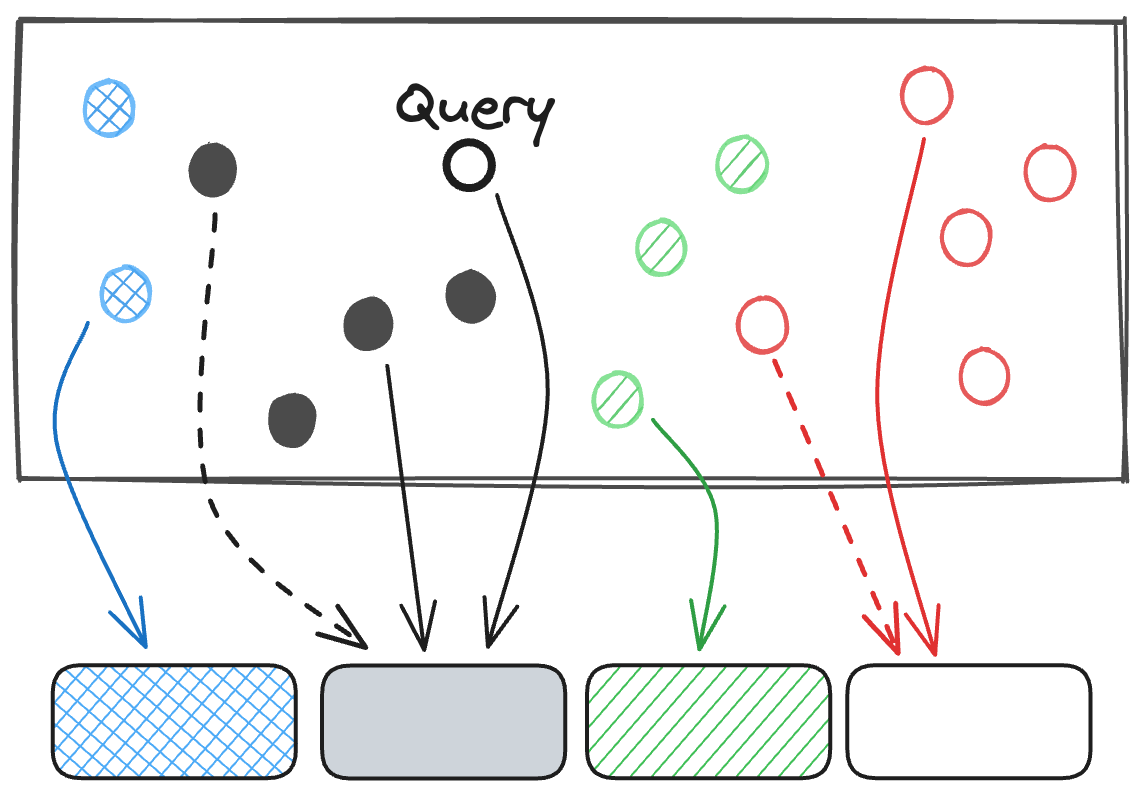
\includegraphics[width=0.49\linewidth]{figures/lsh-intuition-single-mapping.png}
    }
    \subfloat[]{
        \label{figure:lsh:intuition:multi-dimensional}
        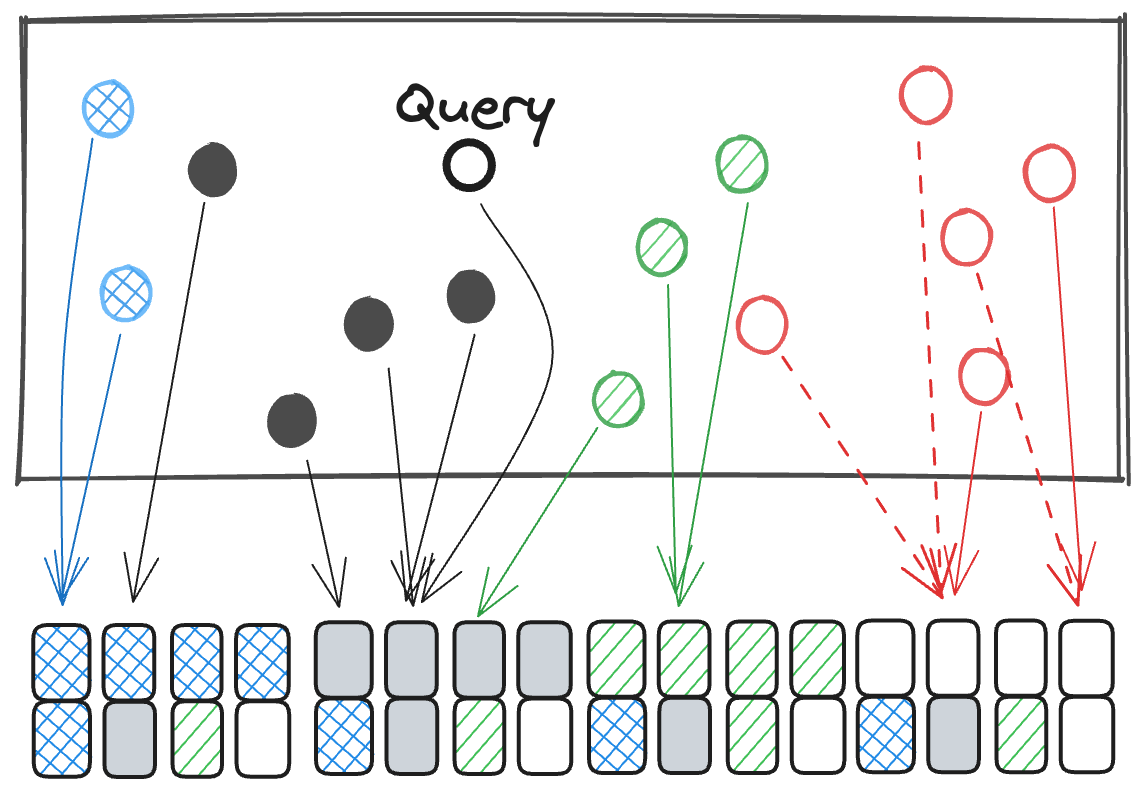
\includegraphics[width=0.49\linewidth]{figures/lsh-intuition-multidimensional-mapping.png}
    }
    \caption{Illustration of Locality Sensitive Hashing. In (a), a function
    $h: \mathbb{R}^2 \rightarrow \{ 1, 2, 3, 4 \}$ maps vectors to four buckets.
    Ideally, when two points are closer to each other, they are more likely to be placed
    in the same bucket. But, as the dashed arrows show, some vectors end up in less-than-ideal
    buckets. When retrieving the top-$k$ vectors for a query $q$, we search through the data
    vectors that are in the bucket $h(q)$. Figure (b) depicts an extension of the framework
    where each bucket is the vector $[h_1(\cdot), h_2(\cdot)]$ obtained from two independent mappings
    $h_1$ and $h_2$.
    }
    \label{figure:lsh:intuition}
\end{figure}

It is easy to extend this setup to ``multi-dimensional'' buckets in the following sense.
If $h_i$'s are independent functions that have the desired property above (i.e., increased
chance of collision with smaller $\delta$), we may define
a bucket in $[b]^\ell$ as the vector mapping $g(\cdot) = [h_1(\cdot), h_2(\cdot), \ldots, h_\ell(\cdot)]$.
Figure~\subref*{figure:lsh:intuition:multi-dimensional} illustrates this extension for $\ell=2$.
The indexing and search procedures work in much the same way. But now, there are
presumably fewer data points in each bucket, and
spurious collisions (i.e., vectors that were mapped to the same bucket 
but that are far from each other according to $\delta$) are less likely to occur.
In this way, we are likely to reduce the overall search time and increase
the accuracy of the algorithm.

Extending the framework even further, we can repeat the process above $L$ times
by constructing independent mappings $g_1(\cdot)$ through $g_L(\cdot)$ from
individual mappings $h_{ij}(\cdot)$ ($1 \leq i \leq L$ and $1 \leq j \leq \ell$),
all of which possessing the property of interest. Because the mappings are independent,
repeating the procedure many times increases the probability of obtaining a high
retrieval accuracy.

That is the essence of the LSH approach to top-$k$ retrieval.
Its key ingredient is the family $\mathcal{H}$ of functions $h_{ij}$'s that have the stated
property \emph{for a given distance function}, $\delta$.
This is the detail that is studied in the remainder of this section.
But before we proceed to define $\mathcal{H}$ for different distance functions,
we will first give a more rigorous description of the algorithm.

\section{Top-\texorpdfstring{$k$}{k} Retrieval with LSH}

Earlier, we described informally the class of mappings that are at the core
of LSH, as hash functions that preserve the distance between points. That is,
the likelihood that such a hash function places two points in the same bucket
is a function of their distance. Let us formalize that notion first in the
following definition, due to~\cite{lsh}.

\begin{definition}[$(r, (1+\epsilon)r, p_1, p_2)$-Sensitive Family]
    \label{definition:lsh:hash-family}
    A family of hash functions $\mathcal{H} = \{ h:\; \mathbb{R}^d \rightarrow [b] \}$
    is called $(r, (1 + \epsilon)r, p_1, p_2)$-sensitive for a distance function $\delta(\cdot, \cdot)$,
    where $\epsilon > 0$ and $0 < p_1, p_2 < 1$, if for any two points $u, v \in \mathbb{R}^d$:
    \begin{itemize}
        \item $\delta(u, v) \leq r \implies \probability_\mathcal{H}\big[ h(u) = h(v) \big] \geq p_1$; and,
        \item $\delta(u, v) > (1 + \epsilon)r \implies \probability_\mathcal{H}\big[ h(u) = h(v) \big] \leq p_2$.
    \end{itemize}
\end{definition}

It is clear that such a family is useful only when $p_1 > p_2$.
We will see examples of $\mathcal{H}$ for different distance functions later in this section.
For the time being, however, suppose such a family of functions exists for any $\delta$ of interest.

The indexing algorithm remains as described before.
Fix parameters $\ell$ and $L$ to be determined later in
this section. Then define the vector function
$g(\cdot) = \big[ h_1(\cdot), h_2(\cdot), \ldots, h_\ell(\cdot) \big]$
where $h_i \in \mathcal{H}$. Now, construct $L$ such functions $g_1$ through $g_L$, and process
the data points in collection $\mathcal{X}$ by evaluating $g_i$'s and placing
them in the corresponding multi-dimensional bucket.

\begin{svgraybox}
In the end, we have effectively
built $L$ tables, each mapping buckets to a list of data points that
fall into them. Note that, each of the $L$ tables holds a copy of the collection,
but where each table organizes the data points differently.
\end{svgraybox}

\subsection{The Point Location in Equal Balls Problem}
Our intuitive description of retrieval using LSH ignored a minor technicality
that we must elaborate in this section. In particular, as is clear from 
Definition~\ref{definition:lsh:hash-family}, a family $\mathcal{H}$ has
a dependency on the distance $r$. That means any instance of the family provides guarantees
only with respect to a specific $r$. Consequently, any index obtained
from a family $\mathcal{H}$, too, is only useful in the context of a fixed $r$.

It appears, then, that the LSH index is not in and of itself sufficient
for solving the $\epsilon$-approximate retrieval problem of
Definition~\ref{definition:flavors:approximate-top-k-retrieval} directly.
But, it is enough for solving an easier \emph{decision problem} that is
known as Point Location in Equal Balls (PLEB), defined as follows:

\begin{definition}[$(r, (1+\epsilon)r)$-Point Location in Equal Balls]
    \label{definition:lsh:pleb}
    For a query point $q$ and a collection $\mathcal{X}$,
    if there is a point $u \in \mathcal{X}$ such that $\delta(q, u) \leq r$,
    return \textsc{Yes} and any point $v$ such that $\delta(q, v) < (1+\epsilon)r$.
    Return \textsc{No} if there are no such points.
\end{definition}

The algorithm to solve the $(r, (1+\epsilon)r)$-PLEB problem for a query point $q$
is fairly straightforward. It involves evaluating $g_i$'s on $q$ and exhaustively searching the
corresponding buckets in order. We may terminate early after visiting at
most $4L$ data points. For every examined data point $u$, the algorithm
returns \textsc{Yes} if $\delta(q, u) \leq (1+\epsilon)r$, and \textsc{No} otherwise.

\subsubsection{Proof of Correctness}

Suppose there exits a point $u^\ast \in \mathcal{X}$ such that
$\delta(q, u^\ast) \leq r$. The algorithm above is correct, in the sense
that it returns a point $u$ with $\delta(q, u) \leq (1+\epsilon)r$,
if we choose $\ell$ and $L$ such that the following two properties hold
with constant probability:
\begin{itemize}
    \item $\exists \;i \in [L] \textit{ s.t. } g_i(u^\ast) = g_i(q)$; and,
    \item $\sum_{j=1}^{L} \Big\lvert \Big( \mathcal{X} \setminus B(q, (1+\epsilon)r) \Big) \cap g_j^{-1}(g_j(q)) \Big\rvert \leq 4L$, where $g_j^{-1}(g_j(q))$ is the set of vectors in bucket $g_j(q)$.
\end{itemize}

The first property ensures that, as we traverse the $L$ buckets associated
with the query point, we are likely to visit either the optimal point $u^\ast$,
or some other point whose distance to $q$ is at most $(1 + \epsilon)r$.
The second property guarantees that with constant probability, there are no more
than $4L$ points in the candidate buckets that are $(1+\epsilon)r$ away from $q$.
As such, we are likely to find a solution before visiting $4L$ points.

We must therefore prove that for some $\ell$ and $L$ the above properties hold.
The following claim shows one such configuration.

\begin{theorem}
    \label{theorem:lsh:pleb-configuration}
    Let $\rho=\ln p_1 / \ln p_2$ and $m=\lvert \mathcal{X} \rvert$.
    Set $L=m^\rho$ and $\ell=\log_{1/p_2} m$. The properties above hold
    with constant probability for a $(r, (1+\epsilon)r, p_1, p_2)$-sensitive LSH family.
\end{theorem}
\begin{proof}
    Consider the first property. We have, from Definition~\ref{definition:lsh:hash-family},
    that, for any $h_i \in \mathcal{H}$:
    \begin{equation*}
        \probability\Big[ h_i(u^\ast) = h_i(q) \Big] \geq p_1.
    \end{equation*}
    That holds simply because $u^\ast \in B(q, r)$. That implies:
    \begin{equation*}
        \probability\Big[ g_i(u^\ast) = g_i(q) \Big] \geq p_1^\ell.
    \end{equation*}
    As such:
    \begin{equation*}
        \probability\Big[ \exists \; i \in [L] \textit{ s.t. } g_i(u^\ast) = g_i(q) \Big] \geq 1 - (1 - p_1^\ell)^L.
    \end{equation*}
    Substituting $\ell$ and $L$ with the expressions given in the theorem gives:
    \begin{equation*}
        \probability\Big[ \exists \; i \in [L] \textit{ s.t. } g_i(u^\ast) = g_i(q) \Big] \geq 1 - (1 - \frac{1}{m^\rho})^{m^\rho} \approx 1 - \frac{1}{e},
    \end{equation*}
    proving that the property of interest holds with constant probability.

    Next, consider the second property. For any point $v$ such that $\delta(q, v) > (1 + \epsilon)r$,
    Definition~\ref{definition:lsh:hash-family} tells us that:
    \begin{align*}
        \probability\Big[ h_i(v) &= h_i(q) \Big] \leq p_2 \implies \probability\Big[ g_i(v) = g_i(q) \Big] \leq p_2^\ell \\
        &\implies \probability\Big[ g_i(v) = g_i(q) \Big] \leq \frac{1}{m} \\
        &\implies \ev\Big[ \Big\lvert v \textit{ s.t. } g_i(v) = g_i(q) \land \delta(q, v) > (1 + \epsilon)r \Big\rvert \;|\; g_i \Big] \leq 1 \\
        &\implies \ev\Big[ \Big\lvert v \textit{ s.t. } g_i(v) = g_i(q) \land \delta(q, v) > (1 + \epsilon)r \Big\rvert \Big] \leq L,
    \end{align*}
    where the last expression follows by the linearity of expectation when applied to all $L$ buckets.
    By Markov's inequality, the probability that there are more than $4L$ points for which $\delta(q, v) > (1+\epsilon)r$
    but that map to the same bucket as $q$ is at most $1/4$. That completes the proof.
\end{proof}

\subsubsection{Space and Time Complexity}

The algorithm terminates after visiting at most $4L$ vectors in the candidate buckets.
Given the configuration of Theorem~\ref{theorem:lsh:pleb-configuration}, this means that
the time complexity of the algorithm for query processing is $\mathcal{O}(d m^\rho)$,
which is sub-linear in $m$.

As for space complexity of the algorithm, note that the index stores each
data point $L$ times. That implies the space required to build an LSH index
has complexity $\mathcal{O}(mL) = \mathcal{O}(m^{1 + \rho})$,
which grows super-linearly with $m$. This growth rate can easily become
prohibitive~\citep{gionis1999hashing,buhler2001lsh-comparison},
particularly because it is often necessary to increase $L$ to reach a higher
accuracy, as the proof of Theorem~\ref{theorem:lsh:pleb-configuration} shows.
How do we reduce this overhead and still obtain sub-linear query time?
That is a question that has led to a flurry of research in the past.

One direction to address that question is to modify the search algorithm so that it visits multiple
buckets from each of the $L$ tables, instead of examining just a single bucket per table.
That is the idea first explored by~\cite{entropyLSH}. In that work, the search
algorithm is the same as in the standard version presented above, but in addition to searching the
buckets for query $q$, it also performs many search operations for perturbed copies of $q$.
While theoretically interesting, their method proves difficult to use in practice.
That is because, the amount of noise needed to perturb a query depends on the distance
of the nearest neighbor to $q$---a quantity that is unknown \emph{a priori}.
Additionally, it is likely that a single bucket may be visited many times over
as we invoke the search procedure on the copies of $q$.

Later,~\cite{multiprobeLSH} refined that theoretical result and presented a method
that, instead of perturbing queries \emph{randomly} and performing multiple hash computations
and search invocations, utilizes a more efficient approach
in deciding which buckets to probe within each table. In particular,
their ``multi-probe LSH'' first finds the bucket associated with $q$, say $g_i(q)$.
It then additionally visits other ``adjacent'' buckets where a bucket is adjacent
if it is more likely to hold data points that are close to the vectors in $g_i(q)$.

The precise way their algorithm arrives at a set of adjacent buckets
depends on the hash family itself. In their work,~\cite{multiprobeLSH}
consider only a hash family for the Euclidean distance, and take advantage
of the fact that adjacent buckets (which are in $[b]^\ell$) differ in each
coordinate by at most $1$---this becomes clearer when we review the LSH family for
Euclidean distance in Section~\ref{section:lsh:euclidean}.
This scheme was shown empirically to reduce by \emph{an order of magnitude}
the total number of hash tables that is required to achieve an accuracy greater
than $0.9$ on high-dimensional datasets.

\medskip

Another direction is to improve the guarantees of the LSH family itself.
As Theorem~\ref{theorem:lsh:pleb-configuration} indicates, $\rho = \log p_1 / \log p_2$
plays a critical role in the efficiency and effectiveness of the search algorithm,
as well as the space complexity of the data structure.
It makes sense, then, that improving $\rho$ leads to smaller space overhead.
Many works have explored advanced LSH families to do just
that~\citep{andoni2008near-optimal,andoni2014beyond,andoni2015cross-polytope-lsh}.
We review some of these methods in more detail later in this chapter.

\subsection{Back to the Approximate Retrieval Problem}
A solution to PLEB of Definition~\ref{definition:lsh:pleb}
is a solution to $\epsilon$-approximate top-$k$ retrieval
only if $r = \delta(q, u^\ast)$, where $u^\ast$ is the $k$-th minimizer
of $\delta(q, \cdot)$. But we do not know the minimal distance in advance!
That begs the question: How does solving the PLEB problem
help us solve the $\epsilon$-approximate retrieval problem?

\cite{lsh} argue that an efficient solution to this decision version of the 
problem leads directly to an efficient solution to the original problem.
In effect, they show that $\epsilon$-approximate retrieval can be reduced
to PLEB. Let us review one simple, albeit inefficient reduction.

Let $\delta_\ast = \max_{u, v \in \mathcal{X}} \delta(u, v)$ and
$\delta^\ast = \min_{u, v \in \mathcal{X}} \delta(u, v)$. Denote by
$\Delta$ the aspect ratio: $\Delta = \delta_\ast / \delta^\ast$.
Now, define a set of distances $\mathcal{R} = \{ (1+\epsilon)^0, (1 + \epsilon)^1, \ldots, \Delta \}$,
and construct $\lvert \mathcal{R} \rvert$ LSH indices for each $r \in \mathcal{R}$.

Retrieving vectors for query $q$ is a matter of performing
binary search over $\mathcal{R}$ to find the minimal
distance such that PLEB succeeds and returns a point $u \in \mathcal{X}$.
That point $u$ is the solution to the $\epsilon$-approximate retrieval
problem! It is easy to see that such a reduction adds to the time complexity
by a factor of $\mathcal{O}(\log \log_{1+\epsilon} \Delta)$, and to the space
complexity by a factor of $\mathcal{O}(\log_{1+\epsilon} \Delta)$.

\section{LSH Families}
We have studied how LSH solves the PLEB problem of Definition~\ref{definition:lsh:pleb},
analyzed its time and space complexity, and reviewed how a solution to PLEB leads
to a solution to the $\epsilon$-approximate top-$k$ retrieval problem of Definition~\ref{definition:flavors:approximate-top-k-retrieval}.
Throughout that discussion, we took for granted the existence of an LSH family
that satisfies Definition~\ref{definition:lsh:hash-family} for a distance function
of interest. In this section, we review example families and unpack their construction
to complete the picture.

\subsection{Hamming Distance}
We start with the simpler case of Hamming distance over the space of binary vectors.
That is, we assume that $\mathcal{X} \subset \{0, 1\}^d$ and $\delta(u, v) = \lVert u - v \rVert_1$,
measuring the number of coordinates in which the two vectors $u$ and $v$ differ.
For this setup, a hash family that maps a vector to one of its coordinates at
random---a technique that is also known as \emph{bit sampling}---is an LSH family~\citep{lsh},
as the claim below shows.

\begin{theorem}
For $\mathcal{X} \subset \{ 0, 1 \}^d$ equipped with the Hamming distance,
the family $\mathcal{H} = \{ h_i \;|\; h_i(u) = u_i, \; 1 \leq i \leq d \}$
is $(r, (1 + \epsilon)r, 1 - r/d, 1 - (1+\epsilon)r/d)$-sensitive.
\end{theorem}
\begin{proof}
    The proof is trivial. For a given $r$ and two vectors $u, v \in \{ 0, 1\}^d$,
    if $\lVert u - v \rVert_1 \leq r$, then $\probability\Big[ h_i(u) \neq h_i(v) \Big] \leq r/d$,
    so that $\probability\Big[ h_i(u) = h_i(v) \Big] \geq 1 - r/d$, and therefore $p_1 = 1 - r/d$.
    $p_2$ is derived similarly.
\end{proof}

\subsection{Angular Distance}
\label{section:lsh:angular}
Consider next the angular distance between two real vectors $u, v \in \mathbb{R}^d$, defined as:
\begin{equation}
    \label{equation:lsh:angular-distance}
    \delta(u, v) = \arccos \Big( \frac{\langle u, v \rangle}{\lVert u \rVert_2 \lVert v \rVert_2} \Big).
\end{equation}

\begin{figure}[t]
    \centering
    \subfloat[Hyperplane LSH]{
        \label{figure:lsh:angular:hyplerplane}
        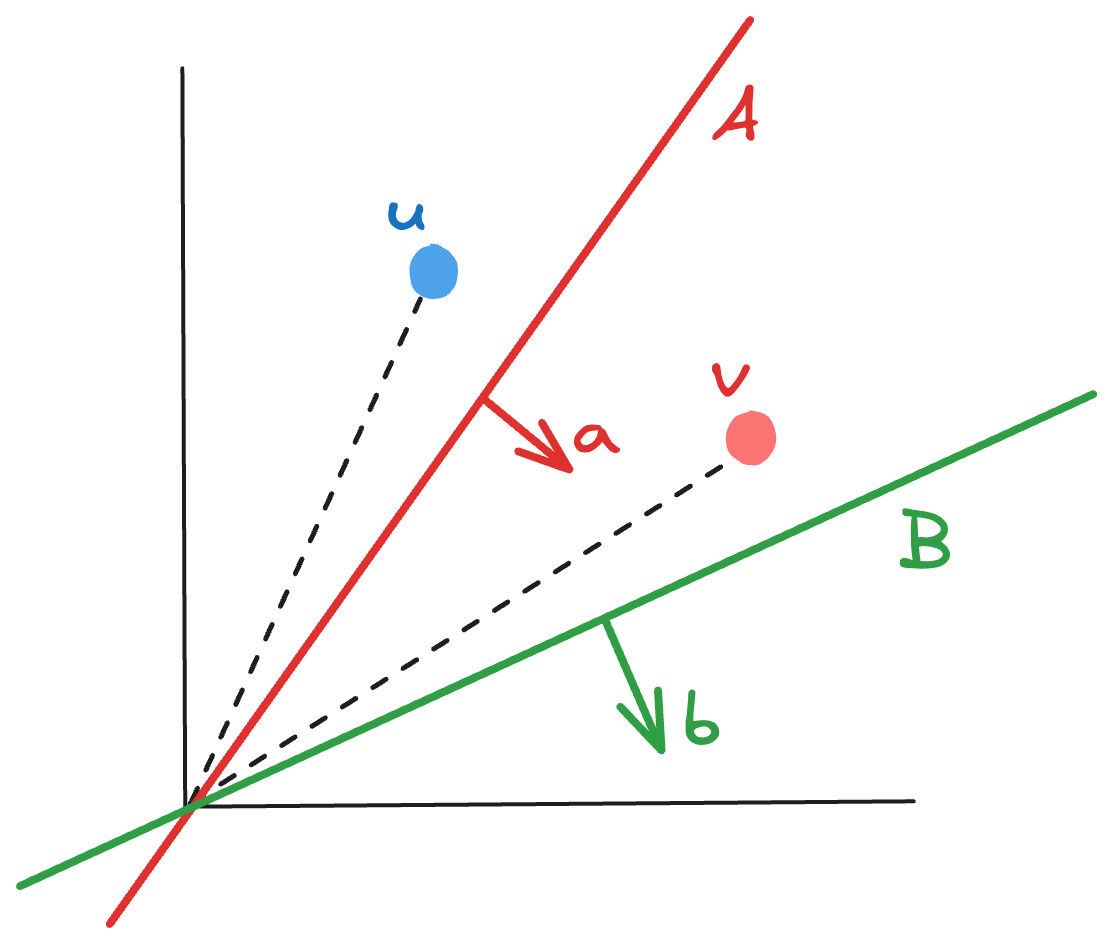
\includegraphics[width=0.4\linewidth]{figures/lsh-hyperplane.png}
    }
    \subfloat[Cross-polytope LSH]{
        \label{figure:lsh:angular:cross-polytope}
        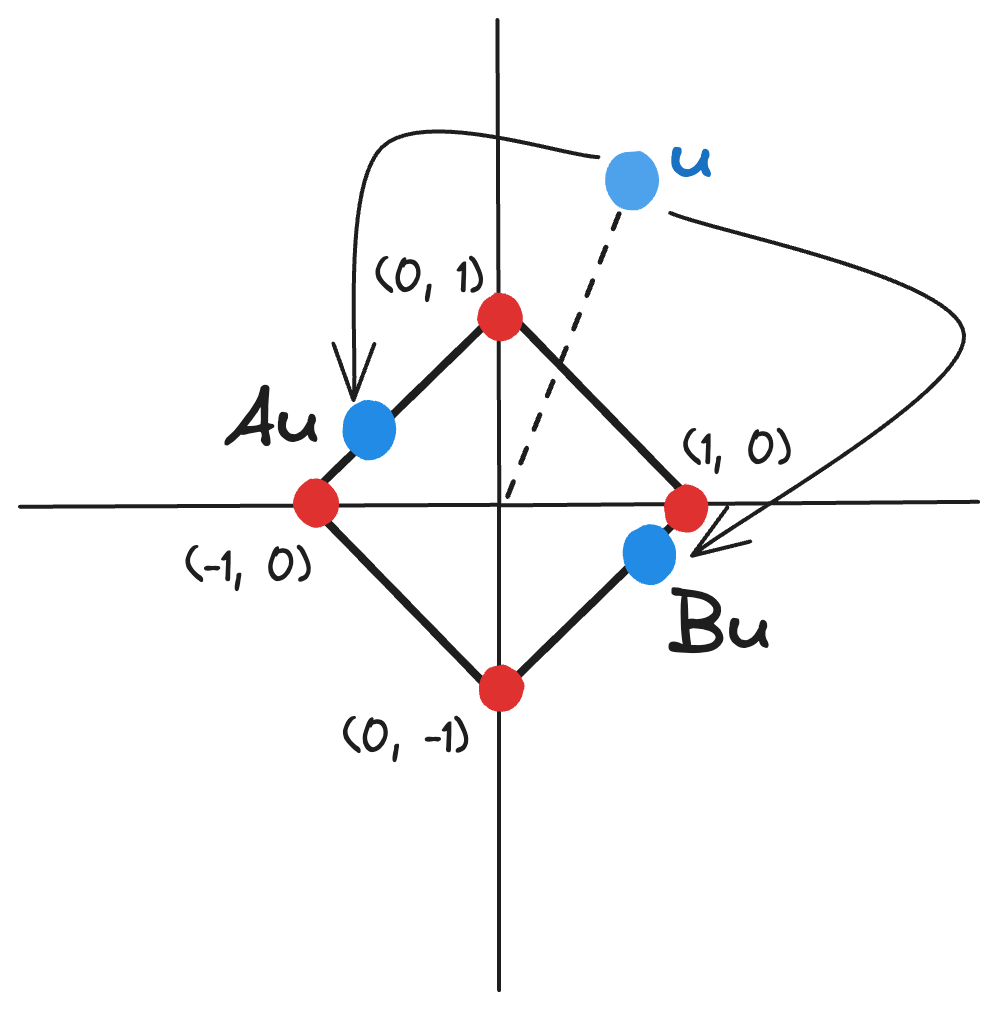
\includegraphics[width=0.4\linewidth]{figures/lsh-cross-polytope.png}
    }
    \caption{Illustration of hyperplane and cross-polytope LSH functions
    for angular distance in $\mathbb{R}^2$. In hyperplane LSH, we draw random
    directions ($a$ and $b$) to define hyperplanes ($A$ and $B$), and record
    $+1$ or $-1$ depending on which side of the hyperplane a vector ($u$ and $v$)
    lies. For example, $h_a(u)=-1$, $h_a(v)=+1$, and $h_b(u)=h_b(v)=-1$. It is easy
    to see that the probability of a hash collision for two vectors $u$ and $v$ correlates
    with the angle between them. A cross-polytope LSH function, on the other hand,
    randomly rotates and normalizes (using matrix $A$ or $B$) the vector ($u$),
    and records the closest standard basis vector as its hash. Note that, the cross-polytope
    is the $L_1$ ball, which in $\mathbb{R}^2$ is a rotated square. As an example,
    $h_A(u) = -e_1$ and $h_B(u) = +e_1$.}
    \label{figure:lsh:angular}
\end{figure}

\subsubsection{Hyperplane LSH}
For this distance function, one simple LSH family is the set
of hash functions that project a vector
onto a randomly chosen direction and record the sign of the projection.
Put differently, a hash function in this family
is characterized by a random hyperplane, which is in turn defined by a unit vector
sampled uniformly at random. When applied to an input vector $u$,
the function returns a binary value (from $\{ -1, 1\}$) indicating on which
side of the hyperplane $u$ is located. This procedure, which is known as \emph{sign random projections}
or \emph{hyperplane LSH}~\citep{charikar2002rounding-algorithms},
is illustrated in Figure~\subref*{figure:lsh:angular:hyplerplane} and
formalized in the following claim.

\begin{theorem}
    For $\mathcal{X} \subset \mathbb{R}^d$ equipped with the angular distance of
    Equation~(\ref{equation:lsh:angular-distance}),
    the family $\mathcal{H} = \{ h_r \;|\; h_r(u) = \textsc{Sign}(\langle r, u \rangle), \; r \sim \mathbb{S}^{d - 1} \}$
    is $(\theta, (1 + \epsilon)\theta, 1 - \theta/\pi, 1 - (1+\epsilon)\theta/\pi)$-sensitive
    for $\theta \in [0, \pi]$, and $\mathbb{S}^{d-1}$ denoting the $d$-dimensional hypersphere.
\end{theorem}
\begin{proof}
    If the angle between two vectors is $\theta$, then the probability that a randomly
    chosen hyperplane lies between them is $\theta / \pi$. As such, the probability that
    they lie on the same side of the hyperplane is $1 - \theta / \pi$. The claim follows.
\end{proof}

\subsubsection{Cross-polytope LSH}
There are a number of other hash families for the angular distance in addition to the basic
construction above. \emph{Spherical LSH}~\citep{andoni2014beyond} is one example, albeit a purely
theoretical one---a single hash computation from that family alone is considerably more expensive
than an exhaustive search over a million data points~\citep{andoni2015cross-polytope-lsh}!

What is known as \emph{Cross-polytope LSH}~\citep{andoni2015cross-polytope-lsh,terasawa2007spherical-lsh}
offers similar guarantees as the Spherical LSH but is a more practical construction.
A function from this family randomly rotates an input vector first, then outputs the closest
signed standard basis vector ($e_i$'s for $1 \leq i \leq d$) as the hash value.
This is illustrated for $\mathbb{R}^2$ in Figure~\subref*{figure:lsh:angular:cross-polytope},
and stated formally in the following result.

\begin{theorem}
    For $\mathcal{X} \subset \mathbb{S}^{d-1}$ equipped with the angular distance of
    Equation~(\ref{equation:lsh:angular-distance}) or equivalently the Euclidean distance,
    the following family constitutes an LSH:
    \begin{equation*}
        \mathcal{H} = \{ h_R \;|\; h_R(u) = \argmin_{e \in \{ \pm e_i \}_{i=1}^d} \lVert e - \frac{Ru}{\lVert R u \rVert_2} \rVert, R \in \mathbb{R}^{d \times d},\; R_{ij} \sim \mathcal{N}(0, 1) \},
    \end{equation*}
    where $\mathcal{N}(0, 1)$ is the standard Gaussian distribution.
    The probability of collision for unit vectors $u, v \in \mathbb{S}^{d-1}$ with $\lVert u - v \rVert < \tau$ is:
    \begin{equation*}
        \ln \frac{1}{\probability\Big[ h_R(u) = h_R(v) \Big]} = \frac{\tau^2}{4 - \tau^2} \ln d + \mathcal{O}_\tau\Big( \ln \ln d \Big).
    \end{equation*}
    Importantly:
    \begin{equation*}
        \rho = \frac{\log p_1}{\log p_2} = \frac{1}{(1 + \epsilon)^2} \frac{4 - (1 + \epsilon)^2 r^2}{4 - r^2} + o(1).
    \end{equation*}
\end{theorem}
\begin{proof}
    We wish to show that, for two unit vectors $u, v \in \mathbb{S}^{d-1}$ with $\lVert u - v \rVert < \tau$,
    the expression above for the probability of a hash collision is correct.
    That, indeed, completes the proof of the theorem itself. To show that, we will
    take advantage of the spherical symmetry of Gaussian random variables---we used this property
    in the proof of Theorem~\ref{theorem:instability:orthogonality-random-vectors}.

    By the spherical symmetry of Gaussians, without loss of generality, we can assume that
    $u = e_1$, the first standard basis, and $v = \alpha e_1 + \beta e_2$,
    where $\alpha^2 + \beta^2 = 1$ (so that $v$ has unit norm) and $(\alpha - 1)^2 + \beta^2 = \tau^2$
    (because the distance between $u$ and $v$ is $\tau$).

    Let us now model the collision probability as follows:
    \begin{align*}
        \probability\Big[ &h(u) = h(v) \Big] = 2d \probability\Big[ h(u) = h(v) = e_1 \Big] \\
        &= 2d \probability_{X, Y \sim \mathcal{N}(0, I)}\Big[ \forall \; i,\; \lvert X_i \rvert \leq X_1 \land
        \lvert \alpha X_i + \beta Y_i \rvert \leq \alpha X_1 + \beta Y_1 \Big] \\
        &= 2d \ev_{X_1, Y_1 \sim \mathcal{N}(0, 1)} \Bigg[ 
            \probability_{X_2, Y_2}\Big[ \lvert X_2 \rvert \leq X_1 \land \lvert \alpha X_2 + \beta Y_2 \rvert \leq \alpha X_1 + \beta Y_1 \Big]^{d-1}
        \Bigg]. \numberthis \label{equation:lsh:cross-polytope:collision-prob}
    \end{align*}
    The first equality is due again to the spherical symmetry of the hash functions
    and the fact that there are $2d$ signed standard basis vectors.
    The second equality simply uses the expressions for $u=e_1$ and $v=\alpha e_1 + \beta e_2$.
    The final equality follows because of the independence of the coordinates of $X$ and $Y$,
    which are sampled from a $d$-dimensional isotropic Gaussian distribution.

    \begin{figure}[t]
        \centering
        \subfloat[]{
            \label{figure:lsh:angular:cross-polytope:planar-set}
            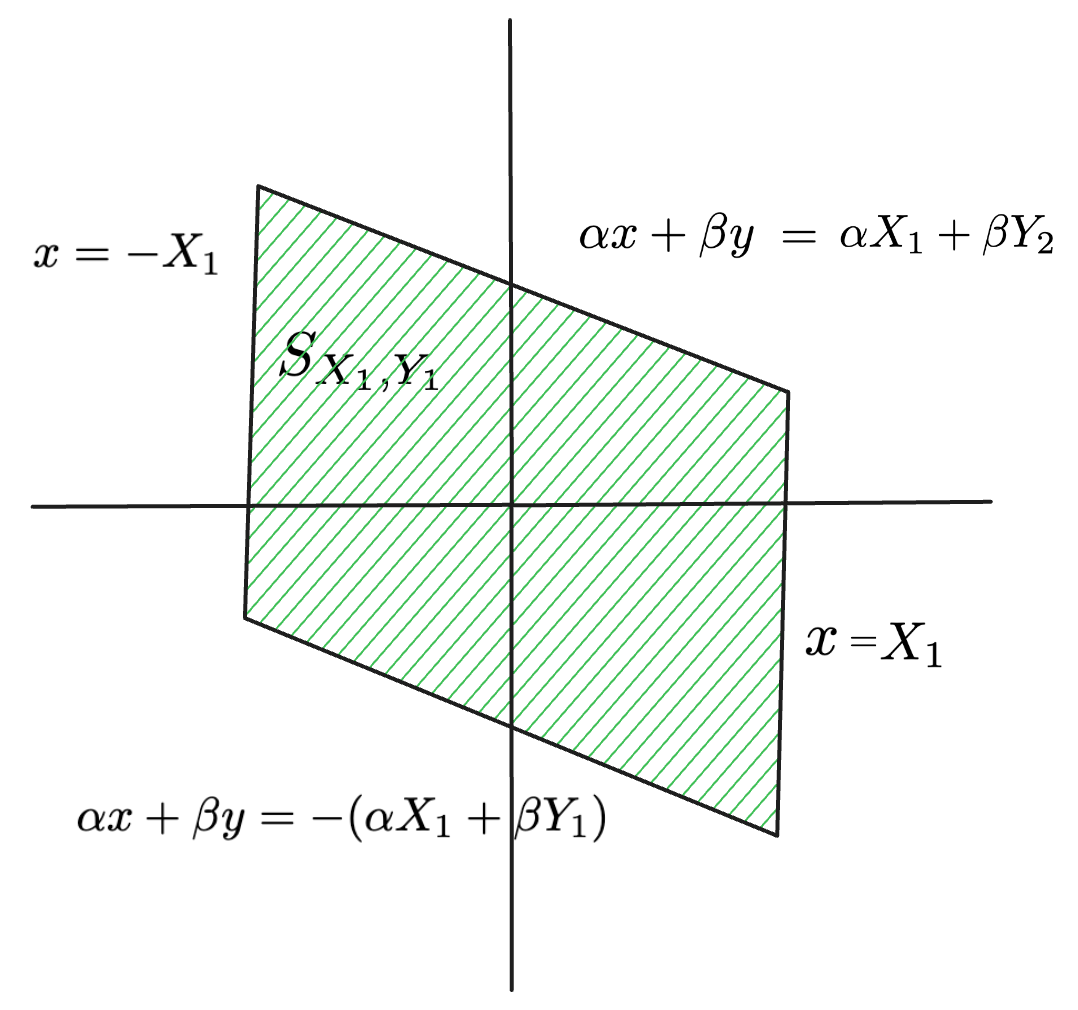
\includegraphics[width=0.4\linewidth]{figures/lsh-crosspolytope-planar-set.png}
        }
        \subfloat[]{
            \label{figure:lsh:angular:cross-polytope:lower-bound}
            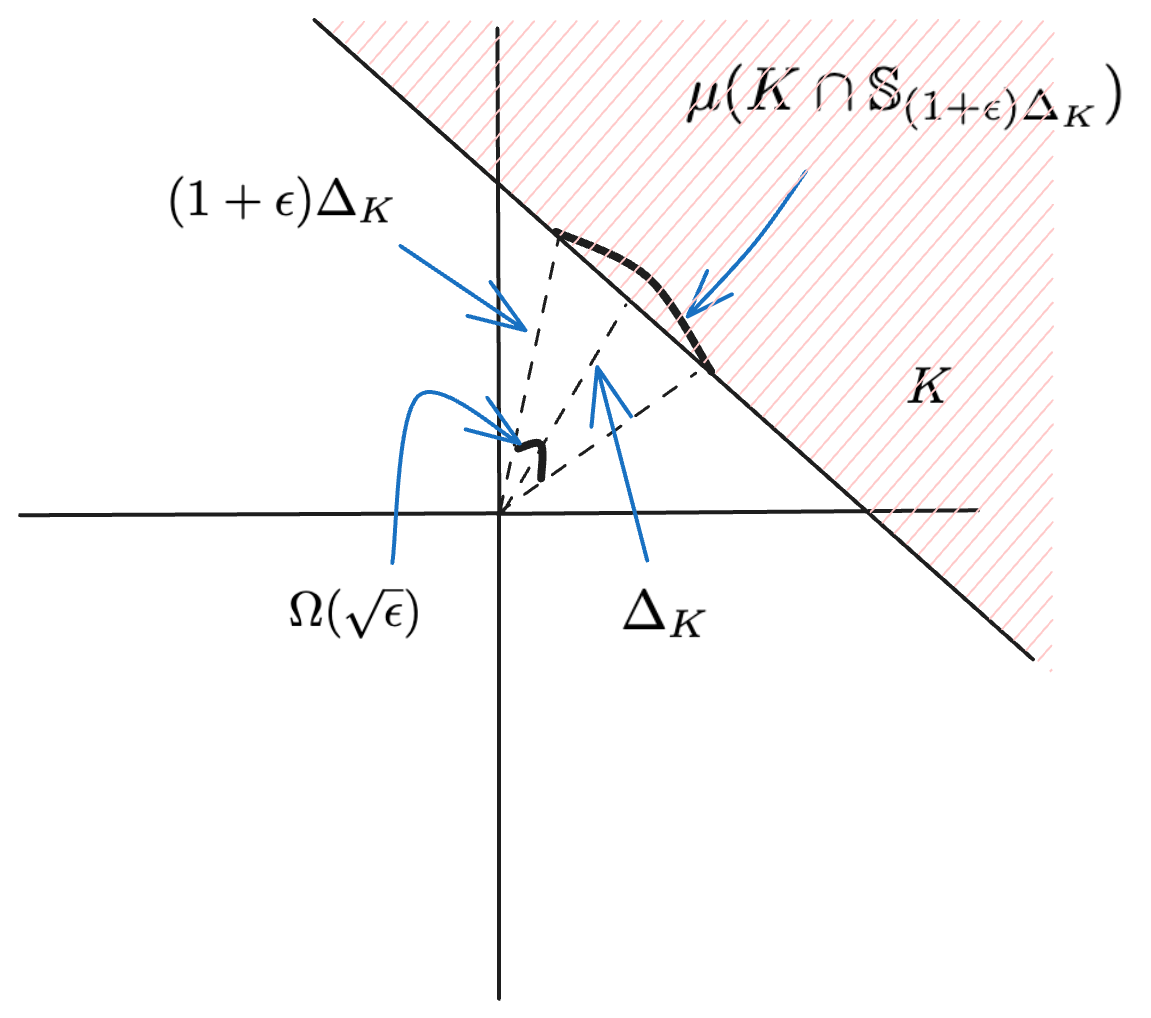
\includegraphics[width=0.4\linewidth]{figures/lsh-crosspolytope-lowerbound.png}
        }
        \caption{Illustration of the set $S_{X_1, Y_1} = \{ \lvert x \rvert \leq X_1 \land \lvert \alpha x + \beta y \rvert \leq \alpha X_1 + \beta Y_1 \}$ in (a). Figure (b) visualizes the derivation of Equation~(\ref{equation:lsh:angular:cross-polytope:proof-lower-bound}).}
        \label{figure:lsh:angular:cross-polytope:proof}
    \end{figure}

    The innermost term in Equation~(\ref{equation:lsh:cross-polytope:collision-prob}) is
    the Gaussian measure of the closed, convex set
    $\{ \lvert x \rvert \leq X_1 \land \lvert \alpha x + \beta y \rvert \leq \alpha X_1 + \beta Y_1 \}$,
    which is a bounded plane in $\mathbb{R}^2$. This set, which we denote by $S_{X_1, Y_1}$,
    is illustrated in Figure~\subref*{figure:lsh:angular:cross-polytope:planar-set}.
    Then we can expand Equation~(\ref{equation:lsh:cross-polytope:collision-prob}) as follows:
    \begin{align}
        \label{equation:lsh:angular:cross-polytope:prob-collision-expanded}
        2d \ev_{X_1, Y_1 \sim \mathcal{N}(0, 1)} &\Bigg[ 
            \probability_{X_2, Y_2}\Big[ S_{X_1, Y_1} \Big]^{d-1}
        \Bigg] \\
        &= 2d \int_0^1 \probability_{X_1, Y_1 \sim \mathcal{N}(0, 1)} \Big[ \probability [ S_{X_1, Y_1} ] \geq t^{\frac{1}{d - 1}} \Big] dt.
    \end{align}
    We therefore need to expand $\probability[S_{X_1, Y_1}]$ in order to complete the expression above.
    The rest of the proof derives that quantity.
    
    \textbf{Step 1}.
    Consider $\probability[S_{X_1, Y_1}] = \mathcal{G}(S_{X_1, Y_1})$, which is the standard Gaussian
    measure of the set $S_{X_1, Y_1}$. In effect, we are interested in $\mathcal{G}(S)$ for some
    bounded convex subset $S \subset \mathbb{R}^2$. We need the following lemma to derive an expression
    for $\mathcal{G}(S)$. But first define $\mu_A(r)$ as the Lebesgue measure of the intersection of a circle
    of radius $r$ ($\mathbb{S}_r$) with the set $A$, normalized by the circumference of $\mathbb{S}_r$,
    so that $0 \leq \mu_A(r) \leq 1$ is a probability measure:
    \begin{equation*}
        \mu_A(r) \triangleq \frac{\mu(A \cap \mathbb{S}_r)}{2 \pi r},
    \end{equation*}
    and denote by $\Delta_A$ the distance from the origin to A (i.e., $\Delta_A \triangleq \inf \{ r > 0 \;|\; \mu_A(r) > 0 \}$).

    \begin{lemma}
        For the closed set $A \subset \mathbb{R}^2$ with $\mu_A(r)$ non-decreasing:
        \begin{equation*}
            \sup_{r > 0} \Big( \mu_A(r) \cdot e^{-r^2/2} \Big) \leq \mathcal{G}(A) \leq e^{-\Delta^2_A/2}.
        \end{equation*}
    \end{lemma}
    \begin{proof}
        The upper-bound can be derived as follows:
        \begin{equation*}
            \mathcal{G}(A) = \int_0^\infty r \mu_A(r) \cdot e^{-r^2/2} dr \leq \int_{\Delta_A}^\infty r e^{-r^2/2} dr = e^{-\Delta_A^2/2}.
        \end{equation*}
        For the lower-bound:
        \begin{equation*}
            \mathcal{G}(A) = \int_0^\infty r \mu_A(r) \cdot e^{-r^2/2} dr \geq \mu_A(r^\prime) \int_{r^\prime}^\infty r e^{-r^2/2} dr =
            \mu_A(r^\prime) e^{-(r^\prime)^2/2},
        \end{equation*}
        for all $r^\prime > 0$. The inequality holds because $\mu_A(\cdot)$ is non-decreasing.
    \end{proof}

    Now, $K^\complement \triangleq S_{X_1, Y_1}$ is a convex set, so for its complement,
    $K \subset \mathbb{R}^2$, $\mu_K(\cdot)$ is non-decreasing.
    Using the above lemma, that fact implies the following for small $\epsilon$:
    \begin{equation*}
        \Omega(\sqrt{\epsilon} \cdot e^{-(1+\epsilon)^2\Delta^2_K/2}) \leq \mathcal{G}(K) \leq e^{-\Delta_K^2/2}.
    \end{equation*}
    The lower-bound uses the fact that $\mu_K \Big( (1 + \epsilon) \Delta_K \Big) = \Omega (\sqrt{\epsilon})$,
    because:
    \begin{equation}
        \label{equation:lsh:angular:cross-polytope:proof-lower-bound}
        \mu(K \cap \mathbb{S}_{(1+\epsilon)\Delta_K}) = (1 + \epsilon) \Delta_K \arccos \Big(
            \frac{\Delta_K}{(1 + \epsilon) \Delta_K} \Big) \approx (1 + \epsilon) \Delta_K \sqrt{\epsilon}.
    \end{equation}
    See Figure~\subref*{figure:lsh:angular:cross-polytope:lower-bound} for a helpful illustration.

    Since we are interested in the measure of $K^\complement = S_{X_1, Y_1}$, we can apply
    the result above directly to obtain:
    \begin{equation}
        \label{equation:lsh:angular:cross-polytope:proof-measure-planar-set}
        1 - e^{-\Delta(u, v)^2/2} \leq \probability [S_{X_1, Y_1}] \leq
        1 - \Omega\Big( \sqrt{\epsilon} \cdot e^{-(1+\epsilon)^2\Delta(u, v)^2/2} \Big),
    \end{equation}
    where we use the notation $\Delta_{K} = \Delta(u, v) = \min \{ u, \alpha u + \beta v \}$.

    \textbf{Step 2}. For simplicity, first consider the side of Equation~(\ref{equation:lsh:angular:cross-polytope:proof-measure-planar-set})
    that does not depend on $\epsilon$,
    and substitute that into Equation~(\ref{equation:lsh:angular:cross-polytope:prob-collision-expanded}).
    We obtain:
    \begin{align*}
        2d \int_0^1 \probability_{X_1, Y_1 \sim \mathcal{N}(0, 1)} &\Big[ \probability [ S_{X_1, Y_1} ] \geq t^{\frac{1}{d - 1}} \Big] dt \\
        &=
        2d \int_0^1 \probability_{X_1, Y_1 \sim \mathcal{N}(0, 1)} \Big[ e^{-\Delta(X_1, Y_1)^2/2} \leq 1 - t^{\frac{1}{d - 1}}  \Big] dt \\
        &= 2d \int_0^1 \probability_{X_1, Y_1 \sim \mathcal{N}(0, 1)} \Big[ \Delta(X_1, Y_1) \geq \sqrt{-2 \log \Big( 1 - t^{\frac{1}{d - 1}} \Big)}  \Big] dt. \numberthis \label{equation:lsh:angular:cross-polytope:prob-collision-noepsilon-substitute}
    \end{align*}

    \textbf{Step 3}. We are left with bounding $\probability[ \Delta(X_1, Y_1) \geq \theta ]$.
    $\Delta(X_1, Y_1) \geq \theta$ is, by definition, the set that is the intersection of two
    half-planes: $X_1 \geq \theta$ and $\alpha X_1 + \beta Y_1 \geq \theta$. If we denote this set
    by $K$, then we are again interested in the Gaussian measure of $K$. For small $\epsilon$,
    we can apply the lemma above to show that:
    \begin{equation}
        \Omega \Big( \epsilon e^{-(1 + \epsilon)^2 \Delta_K^2} \Big) \leq \mathcal{G}(K) \leq e^{-\Delta^2_K /2},
    \end{equation}
    where the constant factor in $\Omega$ depends on the angle between the two half-planes. That is
    because $\mu(K \cap \mathbb{S}_{(1+ \epsilon) \Delta_K})$ is $\epsilon$ times that angle.

    It is easy to see that $\Delta_K^2 = \frac{4}{4 - \tau^2} \cdot \theta^2$, so that we arrive at the following
    for small $\epsilon$ and every $\theta \geq 0$:
    \begin{equation}
        \label{equation:lsh:angular:cross-polytope:proof-bound-delta}
        \Omega_\tau \Big( \epsilon \cdot e^{-(1 + \epsilon)^2 \cdot \frac{4}{4 - \tau^2}\cdot \frac{\theta^2}{2}} \Big) \leq
        \probability_{X_1, Y_1 \sim \mathcal{N}(0, 1)} \Big[ \Delta(X_1, Y_1) \geq \theta \Big] \leq
        e^{- \frac{4}{4 - \tau^2}\cdot \frac{\theta^2}{2}}.
    \end{equation}

    \textbf{Step 4}. Substituting Equation~(\ref{equation:lsh:angular:cross-polytope:proof-bound-delta}) into
    Equation~(\ref{equation:lsh:angular:cross-polytope:prob-collision-noepsilon-substitute}) yields:
    \begin{align*}
        2d \int_0^1 \probability_{X_1, Y_1 \sim \mathcal{N}(0, 1)} &\Big[ \Delta(X_1, Y_1) \geq \sqrt{-2 \log \Big( 1 - t^{\frac{1}{d - 1}} \Big)}  \Big] dt \\
        &= 2d \int_0^1 \Big( 1 - t^{\frac{1}{d - 1}} \Big)^{\frac{4}{4 - \tau^2}}dt \\
        &= 2d(d-1) \int_0^1 (1 - x)^{\frac{4}{4 - \tau^2}} x^{d-2} dt \\
        &= 2d (d - 1) B\Big( \frac{8 - \tau^2}{4 - \tau^2}; d - 1 \Big) \\
        &= 2d \Theta_\tau(1) d^{-\frac{4}{4 - \tau^2}},
    \end{align*}
    where $B$ denotes the Beta function and the last step uses the Stirling approximation.

    The result above can be expressed as follows:
    \begin{equation*}
        \ln \frac{1}{\probability [ h(u) = h(v)]} = \frac{\tau^2}{4 - \tau^2} \ln d \pm \mathcal{O}_\tau(1).
    \end{equation*}

    \textbf{Step 5}. Repeating Steps 2 through 4 with the expressions that involve $\epsilon$ in
    Equations~(\ref{equation:lsh:angular:cross-polytope:proof-measure-planar-set})
    and~(\ref{equation:lsh:angular:cross-polytope:proof-bound-delta}) gives the desired result.
\end{proof}

Finally, \cite{andoni2015cross-polytope-lsh} show that,
instead of applying a random rotation using Gaussian random variables, it is sufficient to
use a pseudo-random rotation based on Fast Hadamard Transform. In effect,
they replace the random Gaussian matrix $R$ in the construction above with
three consecutive applications of $HD$, where $H$ is the Hadamard matrix
and $D$ is a random diagonal sign matrix (where the entries on the diagonal take
values from $\{\pm 1\}$).

\subsection{Euclidean Distance}
\label{section:lsh:euclidean}
\cite{datar2004pstable-lsh} proposed the first LSH family for the Euclidean distance,
$\delta(u, v) = \lVert u - v \rVert_2$. Their construction relies on the notion of
\emph{$p$-stable distributions} which we define first.

\begin{definition}[$p$-stable Distribution]
    A distribution $\mathcal{D}_p$ is said to be $p$-stable if $\sum_{i=1}^n \alpha_i Z_i$,
    where $\alpha_i \in \mathbb{R}$ and $Z_i \sim \mathcal{D}_p$, has the same distribution
    as $\lVert \alpha \rVert_p Z$, where $\alpha = [\alpha_1, \alpha_2, \ldots, \alpha_n ]$
    and $Z \sim \mathcal{D}_p$. As an example, the Gaussian distribution is $2$-stable.
\end{definition}

Let us state this property slightly differently so it is easier to understand its
connection to LSH. Suppose we have an arbitrary vector $u \in \mathbb{R}^d$.
If we construct a $d$-dimensional random vector $\alpha$ whose coordinates are independently sampled from
a $p$-stable distribution $\mathcal{D}_p$, then the inner product $\langle \alpha, u \rangle$ is
distributed according to $\lVert u \rVert_p Z$ where $Z \sim \mathcal{D}_p$.
By linearity of inner product, we can also see that $\langle \alpha, u \rangle - \langle \alpha, v \rangle$,
for two vectors $u, v \in \mathbb{R}^d$, is distributed as $\lVert u - v \rVert_p Z$.
This particular fact plays an important role in the proof of the following result.

\begin{theorem}
    For $\mathcal{X} \subset \mathbb{R}^d$ equipped with the Euclidean distance,
    a $2$-stable distribution $\mathcal{D}_2$, and the uniform distribution $U$ over
    the interval $[0, r]$,
    the following family is $(r, (1 + \epsilon)r, p(r), p((1 + \epsilon) r))$-sensitive:
    \begin{equation*}
     \mathcal{H} = \{ h_{\alpha, \beta} \;|\; h_{\alpha, \beta}(u) = 
    \lfloor \frac{\langle \alpha, u \rangle + \beta }{r} \rfloor, \; \alpha \in \mathbb{R}^d,\; \alpha_i \sim \mathcal{D}_2,\;
    \beta \sim U[0, r] \},
    \end{equation*}
    where:
    \begin{equation*}
        p(x) = \int_{t=0}^{r} \frac{1}{x} f\Big( \frac{t}{x} \Big) \Big( 1 - \frac{t}{r} \Big) dt,
    \end{equation*}
    and $f$ is the probability density function of the \emph{absolute value} of $\mathcal{D}_2$.
\end{theorem}
\begin{proof}
    The key to proving the claim is modeling the probability of a hash collision for two
    arbitrary vectors $u$ and $v$: $\probability\Big[ h_{\alpha, \beta}(u) = h_{\alpha, \beta}(v) \Big]$.
    That event can be expressed as follows:
    \begin{align*}
        \probability\Big[ h_{\alpha, \beta}(u) &= h_{\alpha, \beta}(v) \Big] = 
        \probability\Big[ \Big\lfloor \frac{\langle \alpha, u \rangle + \beta}{r} \Big\rfloor =  \Big\lfloor \frac{\langle \alpha, v \rangle + \beta}{r} \Big\rfloor \Big] \\
        &= \probability\Big[ \underbrace{\lvert \langle \alpha, u - v \rangle \rvert < r}_{\textit{Event A}} \;\land \\
        &\underbrace{\langle \alpha, u \rangle + \beta \textit{ and } \langle \alpha, v \rangle + \beta \textit{ do not straddle an integer }}_{\textit{Event B}} \Big].
    \end{align*}
    Using the $2$-stability of $\alpha$, Event A is equivalent to $\lVert u - v \rVert_2 \lvert Z \rvert < r$,
    where $Z$ is drawn from $\mathcal{D}_2$. The probability of the complement of Event B is simply
    the ratio between $\langle \alpha, u - v \rangle$ and $r$. Putting all that together, we obtain that:
    \begin{align*}
        \probability\Big[ h_{\alpha, \beta}(u) = h_{\alpha, \beta}(v) \Big] &= 
        \int_{z = 0}^{\frac{r}{\lVert u - v \rVert_2}} f(z) \Big( 1 - \frac{z \lVert u - v \rVert_2}{r} \Big) dz \\
        &= \int_{t = 0}^{r} \frac{1}{\lVert u - v \rVert_2} f(\frac{t}{\lVert u - v \rVert_2}) \Big( 1 - \frac{t}{r} \Big) dt,
    \end{align*}
    where we derived the last equality by the variable change $t = z \lVert u - v \rVert_2$.
    Therefore, if $\lVert u - v \rVert \leq x$:
    \begin{equation*}
        \probability\Big[ h_{\alpha, \beta}(u) = h_{\alpha, \beta}(v) \Big] \geq
        \int_{t = 0}^{r} \frac{1}{x} f(\frac{t}{x}) \Big( 1 - \frac{t}{r} \Big) dt = p(x).
    \end{equation*}
    It is easy to complete the proof from here.
\end{proof}

\subsection{Inner Product}
\label{section:lsh:ip}

Many of the arguments that establish the existence of an LHS family for a distance function
of interest rely on triangle inequality. Inner product as a measure of similarity, however,
does not enjoy that property. As such, developing an LSH family for inner product requires
that we somehow transform the problem from MIPS to NN search or MCS search,
as was the case in Chapter~\ref{chapter:branch-and-bound}.

Finding the right transformation that results in improved hash quality---as determined by
$\rho$---is the question that has been explored by several works in the
past~\citep{Neyshabur2015lsh-mips,shrivastava2015alsh,shrivastava2014alsh,yan2018norm-ranging-lsh}.

Let us present a simple example. Note that, we may safely assume that queries are unit
vectors (i.e., $q \in \mathbb{S}^{d-1}$), because the norm of the query does not
change the outcome of MIPS. 

Now, define the transformation $\phi_d: \mathbb{R}^d \rightarrow \mathbb{R}^{d + 1}$,
first considered by~\cite{xbox-tree}, as follows: $\phi_d(u) = [u, \; \sqrt{1 - \lVert u \rVert_2^2}]$.
Apply this transformation to data points in $\mathcal{X}$.
Clearly, $\lVert \phi_d(u) \rVert_2 = 1$ for all $u \in \mathcal{X}$.
Separately, pad the query points with a single $0$: $\phi_q(v) = [v; 0] \in \mathbb{R}^{d+1}$.

We can immediately verify that $\langle q, u \rangle = \langle \phi_q(q), \phi_d(u) \rangle$
for a query $q$ and data point $u$.
But by applying the transformations $\phi_d(\cdot)$ and $\phi_q(\cdot)$,
we have reduced the problem to MCS! As such, we may use any of existing LSH families
that we have seen for angular distance in Section~\ref{section:lsh:angular} for MIPS.

\medskip

There has been much debate over the suitability of the standard LSH framework
for inner product, with some works extending the framework to what is known as \emph{asymmetric}
LSH~\citep{shrivastava2014alsh,shrivastava2015alsh}. It turns out, however, that none of that
is necessary. In fact, as~\cite{Neyshabur2015lsh-mips} argued formally and demonstrated empirically,
the simple scheme we described above sufficiently addresses MIPS.

\section{Closing Remarks}
Much like branch-and-bound algorithms, an LSH approach to top-$k$ retrieval
rests on a solid theoretical foundation. There is a direct link between all that is
developed theoretically and the accuracy of an LSH-based top-$k$ retrieval system.

Like tree indices, too, the LSH literature is arguably mature.
There is therefore not a great deal of open questions left to investigate in its foundation,
with many recent works instead exploring learnt hash functions or
its applications in other domains.

What remains open and exciting in the context of top-$k$ retrieval, however,
is the possibility of extending the theory of LSH to explain the success of
other retrieval algorithms. We will return to this discussion in
Chapter~\ref{chapter:ivf}.

\bibliographystyle{abbrvnat}
\bibliography{biblio}
